

\documentclass{article}

\usepackage[utf8]{inputenc}
\usepackage{multicol}
\usepackage{graphicx}
\usepackage{float}
\usepackage{indentfirst}
\usepackage{amsmath}


\begin{document}
\begin{section}{NPS}
We are using SERPENT in external source mode to simulate a hybrid system fusion-fission. The geometry simulated is based on concentrically spheres, where there are nine zones filled with the RFS with thorium and ten zones with coolant Li$_{17}$Pb$_{83}$. The source was produced by the D-T fusion reaction generating neutrons of $14.1$ MeV and placed in the central sphere with a radius of 250 cm, as shown in Figure \ref{fusion}. 

\begin{figure}[htb!]
\centering

\includegraphics[scale=0.4]{fusion.png}
\caption{Fusion system geometry.}
\label{fusion}
\end{figure}

We are having problems to understand how NPS value influences the results of k$_{eff}$(analog) in those simulations. It was noticed that the values of k$_{eff}$(analog) increases considerably when the value of NPS is also increased. Even for high values of NPS (larger than 500000), the values of  k$_{eff}$(analog) obtained for various NPS are considerably different. Table \ref{NPS} shows the k$_{eff}$(analog) values obtained for several NPS values. 

\begin{table}[htb!]
\caption{k$_{eff}$ Results for different NPS}
\label{NPS}
\centering
\vspace{0.5cm}
\begin{tabular}{c|c|c}\hline
NPS & k$_{eff}$(analog) & 95\% confidence interval\\ \hline

$10000$ & $0.59490$ & $0.53182-0.65798$\\ \hline
$20000$ & $0.69282$ & $0.64750-0.73802$\\ \hline
$30000$ & $0.74796$ & $0.71240-0.78352$\\ \hline
$40000$ & $0.77101$ & $0.74249-0.79953$\\ \hline
$50000$ & $0.76816$ & $0.73942-0.79690$\\ \hline
$60000$ & $0.79388$ & $0.76734-0.82042$\\ \hline
$100000$ & $0.82596$ & $0.80478-0.84714$\\ \hline
${\bf 500000}$ & $0.88611$ & $0.87775-0.89447$\\ \hline
${\bf 1000000}$ & $0.89095$ & $0.88547-0.89643$\\ \hline
${\bf 10000000}$ & $0.90109$ & $0.89905-0.90313$\\ \hline
${\bf 20000000}$ & $0.90142$ & $0.90012-0.90272$\\ \hline
\end{tabular}
\end{table}

Similar behavior is verified when we use SERPENT to simulate ADS. Is there a limit inferior to NPS?
\end{section}

\newpage
\begin{section}{Computational Time}

Four ADS cases were simulated using SERPENT Code:  GANEX fuel spiked with 50\% of thorium (case 1), GANEX fuel spiked with 50\% of depleted uranium (case 2), UREX$+$ fuel spiked with 50\% of thorium (case 3) and UREX$+$ fuel spiked with 50\% of depleted uranium (case 4). In both cases, the subcritical core is a cylinder of $12.0m^3$ filled with a hexagonal lattice formed by 120 $^{232}ThO_2$ rods (gray fuel rods) and 36 rods with reprocessed fuel (green fuel rods). The lead was used as a coolant and as a reflector. The simulated geometry is shown in Fig. \ref{geo}.


%%%%%%%%%%%%%%%%%%%%%%%%%%%%%%%%%%%%%%%%%%%%%%%%%%%%%%%%%%%%%%%%%%%%%%%%%%%%%%%%%%%%%%%%%%%%%%%%%%%%%%%%%%%%%%%%%%%%%%%%%%%%%%%%%%%%%%%%%%%%%%%%%%%%%%%%%%%%
\begin{figure}[htb!]
\centering
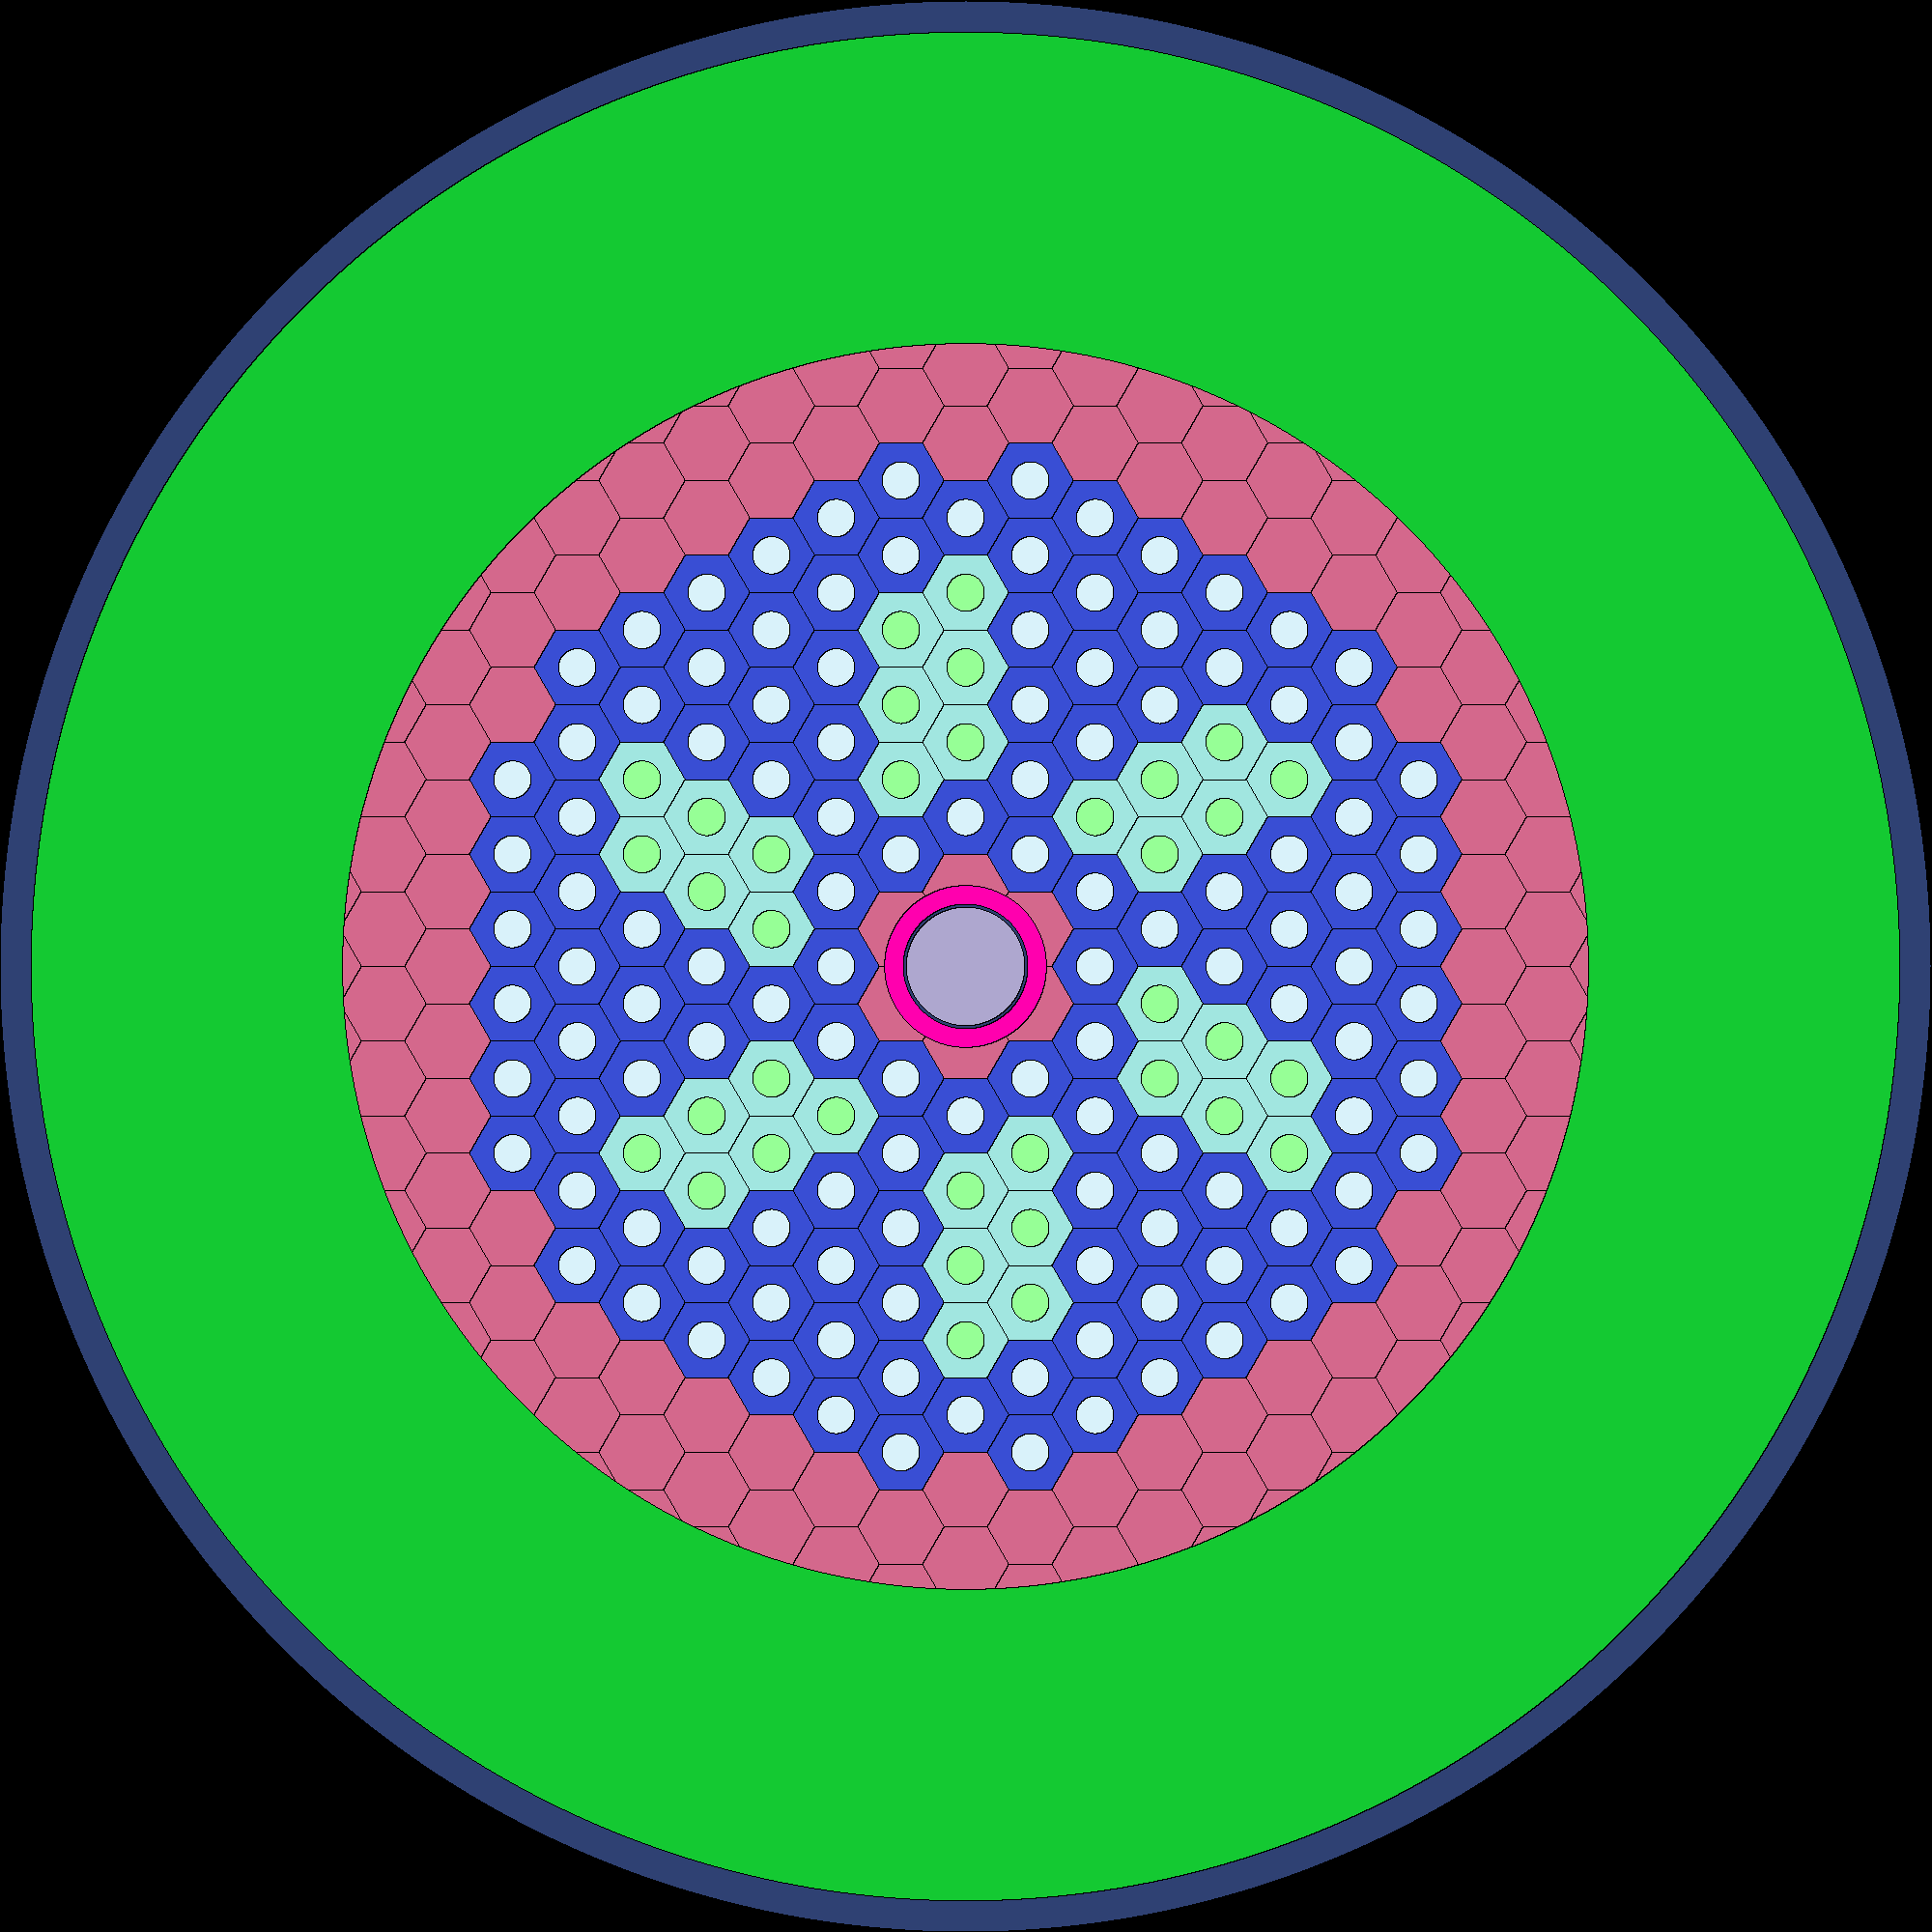
\includegraphics[scale=0.1]{50Th_geom1.png}
\caption{Horizontal cross section of the ADS.}
\label{geo}
\end{figure}
%%%%%%%%%%%%%%%%%%%%%%%%%%%%%%%%%%%%%%%%%%%%%%%%%%%%%%%%%%%%%%%%%%%%%%%%%%%%%%%%%%%%%%%%%%%%%%%%%%%%%%%%%%%%%%%%%%%%%%%%

For all materials, cross-sections libraries available in SERPENT were specified at working temperature, wich is 1200 K for containing fissile/fissionable material and 900 K for the remaining regions. The parameters for the simulated particle population in external source mode were set to run 2 million source neutrons. The burnup calculation was performed for 10 years with the same parameters in both cases and all nuclides were included in the dep.m output file.  

Table \ref{time} shows the computational time spent to perform each case. When we use reprocessed fuel spiked with uranium the computational time is considerably longer.

\begin{table}[htb!]
\caption{Computational time}
\label{time}
\centering
\vspace{0.5cm}
\begin{tabular}{l|c}\hline   
Case & Computational time\\ \hline
Case 1 (GANEX + Th) & $194h:18m:44s$\\ \hline
Case 2 (GANEX + U) & $287h:25m:16s $\\ \hline
Case 3 (UREX + Th) & $208h:41m:45s $\\ \hline
Case 4 (UREX + U) & $300h:43m:54s $\\ \hline
\end{tabular}
\end{table}



\end{section}

\end{document}
